\documentclass{article}
\usepackage{amsmath}
\usepackage{graphicx}
\usepackage{float}
\usepackage{caption}
\usepackage{siunitx}

\title{Statistická analýza váhy policistů}
\author{Vaše jméno}
\date{\today}

\begin{document}

\maketitle

\section{Úvod}
Tento dokument obsahuje statistickou analýzu kvantitativní proměnné – váhy policistů. Použité metody zahrnují výpočet deskriptivních statistik, měření variability a vizualizaci dat pomocí histogramu a boxplotu. Každá statistika je doplněna o vzorce a podrobnou interpretaci.

\section{Data}
Data obsahují váhy policistů v kilogramech. Proměnná \texttt{weight} je numerická a spojitá.

\section{Deskriptivní statistiky}

\subsection{Aritmetický průměr}
Aritmetický průměr je definován jako součet všech hodnot dělený počtem hodnot:
\[
\bar{x} = \frac{1}{n} \sum_{i=1}^{n} x_i
\]
Výsledek:
\[
\bar{x} = \SI{78.448}{\kilo\gram}
\]
\textbf{Interpretace:} Průměrná váha policistů je \SI{78.448}{\kilo\gram}. Tato hodnota je citlivá na extrémní hodnoty (outliery).

\subsection{Vážený průměr}
Vážený průměr je definován jako:
\[
\bar{x}_w = \frac{\sum_{i=1}^{n} w_i x_i}{\sum_{i=1}^{n} w_i}
\]
kde \( w_i \) jsou váhy jednotlivých hodnot. V našem případě jsou všechny váhy stejné, proto je vážený průměr shodný s aritmetickým průměrem:
\[
\bar{x}_w = \SI{78.448}{\kilo\gram}
\]

\subsection{Upravený průměr}
Upravený průměr (trimmed mean) odstraní určité procento nejnižších a nejvyšších hodnot, aby se omezil vliv outlierů. Pro \( \alpha = 0.10 \):
\[
\bar{x}_{\text{trim}} = \frac{1}{n - 2k} \sum_{i=k+1}^{n-k} x_{(i)}
\]
kde \( k = \lfloor \alpha n \rfloor \). Výsledek:
\[
\bar{x}_{\text{trim}} = \SI{77.9025}{\kilo\gram}
\]
\textbf{Interpretace:} Po odstranění 10 \% nejnižších a nejvyšších hodnot je průměrná váha \SI{77.9025}{\kilo\gram}. To naznačuje, že extrémní hodnoty mírně zvyšují aritmetický průměr.

\subsection{Medián}
Medián je prostřední hodnota seřazených dat:
\[
\text{Medián} = x_{(n+1)/2} \quad \text{(pro lichý počet dat)}
\]
Výsledek:
\[
\text{Medián} = \SI{77.95}{\kilo\gram}
\]
\textbf{Interpretace:} Polovina policistů má váhu nižší než \SI{77.95}{\kilo\gram} a polovina vyšší. Medián je robustní vůči extrémním hodnotám.

\subsection{Huberův odhad}
Huberův odhad je robustní metoda kombinující prvky aritmetického průměru a mediánu. Pro výpočet se používá iterativní algoritmus, který minimalizuje kombinaci kvadratické a lineární ztrátové funkce. Výsledek:
\[
\text{Huberův odhad} = \SI{78.17315}{\kilo\gram}
\]
\textbf{Interpretace:} Tento odhad je méně ovlivněn extrémy než aritmetický průměr, ale stále zohledňuje informace z celého rozsahu dat.

\subsection{Tukeyho čísla}
Tukeyho čísla zahrnují minimum, první kvartil (Q1), medián (Q2), třetí kvartil (Q3) a maximum:
\[
\text{Tukeyho čísla} = (\SI{55.10}{\kilo\gram}, \SI{69.60}{\kilo\gram}, \SI{77.95}{\kilo\gram}, \SI{87.00}{\kilo\gram}, \SI{102.20}{\kilo\gram})
\]
\textbf{Interpretace:} 
\begin{itemize}
    \item Minimální váha: \SI{55.10}{\kilo\gram}
    \item 25 \% policistů má váhu nižší než \SI{69.60}{\kilo\gram}
    \item Medián: \SI{77.95}{\kilo\gram}
    \item 75 \% policistů má váhu nižší než \SI{87.00}{\kilo\gram}
    \item Maximální váha: \SI{102.20}{\kilo\gram}
\end{itemize}

\section{Měření variability}

\subsection{Interquartile Range (IQR)}
IQR je rozdíl mezi třetím a prvním kvartilem:
\[
\text{IQR} = Q3 - Q1 = \SI{87.00}{\kilo\gram} - \SI{69.60}{\kilo\gram} = \SI{17.15}{\kilo\gram}
\]
\textbf{Interpretace:} Střední 50 \% dat má rozptyl \SI{17.15}{\kilo\gram}.

\subsection{Rozptyl}
Rozptyl je průměrný kvadratický rozdíl od aritmetického průměru:
\[
\sigma^2 = \frac{1}{n} \sum_{i=1}^{n} (x_i - \bar{x})^2
\]
Výsledek:
\[
\sigma^2 = \SI{131.1711}{\kilo\gram^2}
\]
\textbf{Interpretace:} Průměrný kvadratický rozdíl od průměru je \SI{131.1711}{\kilo\gram^2}. Vyšší rozptyl indikuje větší variabilitu dat.

\subsection{Směrodatná odchylka}
Směrodatná odchylka je odmocnina rozptylu:
\[
\sigma = \sqrt{\sigma^2} = \SI{11.453}{\kilo\gram}
\]
\textbf{Interpretace:} Průměrná odchylka od průměru je \SI{11.453}{\kilo\gram}. Vyšší hodnota znamená větší rozptyl dat.

\subsection{Variační koeficient}
Variační koeficient je poměr směrodatné odchylky k průměru:
\[
\text{CV} = \left( \frac{\sigma}{\bar{x}} \right) \times 100 = \SI{14.59947}{\percent}
\]
\textbf{Interpretace:} Relativní variabilita dat je \SI{14.59947}{\percent}. Tato hodnota umožňuje srovnání variability mezi různými soubory dat.

\subsection{Mediánová absolutní odchylka (MAD)}
MAD je robustní měření variability:
\[
\text{MAD} = \text{med}(|x_i - \text{med}(x)|) = \SI{12.75036}{\kilo\gram}
\]
\textbf{Interpretace:} Průměrná absolutní odchylka od mediánu je \SI{12.75036}{\kilo\gram}. Tato metrika je méně citlivá na extrémy.

\section{Šikmost a špičatost}

\subsection{Šikmost}
Šikmost měří asymetrii rozdělení:
\[
\text{Šikmost} = \frac{1}{n} \sum_{i=1}^{n} \left( \frac{x_i - \bar{x}}{\sigma} \right)^3 = 0.2932968
\]
\textbf{Interpretace:} Pozitivní šikmost naznačuje, že data jsou mírně nakloněna k nižším hodnotám.

\subsection{Špičatost}
Špičatost měří koncentraci hodnot kolem modu a výskyt extrémních hodnot:
\[
\text{Špičatost} = \frac{1}{n} \sum_{i=1}^{n} \left( \frac{x_i - \bar{x}}{\sigma} \right)^4 - 3 = -0.8435781
\]
\textbf{Interpretace:} Negativní špičatost naznačuje, že distribuce má "lehké konce" (nižší výskyt extrémních hodnot).

\section{Vizualizace}

\subsection{Histogram}
Histogram ukazuje frekvenční rozdělení váhy policistů. 
Většina hodnot se nachází mezi \SI{70}{\kilo\gram} a \SI{90}{\kilo\gram}, což potvrzuje mírně pozitivní šikmost.

\begin{figure}[H]
    \centering
    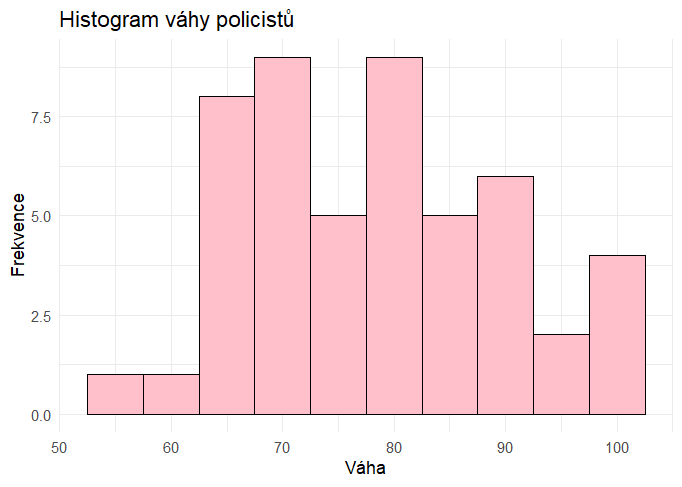
\includegraphics[width=0.8\textwidth]{histogram.png}
    \caption{Histogram váhy policistů}
    \label{fig:histogram}
\end{figure}

\subsection{Boxplot}
Boxplot zobrazuje Tukeyho čísla a potvrzuje, že střední 50 \% dat je mezi \SI{69.60}{\kilo\gram} a \SI{87.00}{\kilo\gram}. Nejsou zde viditelné extrémní odlehlé hodnoty.

\begin{figure}[H]
    \centering
    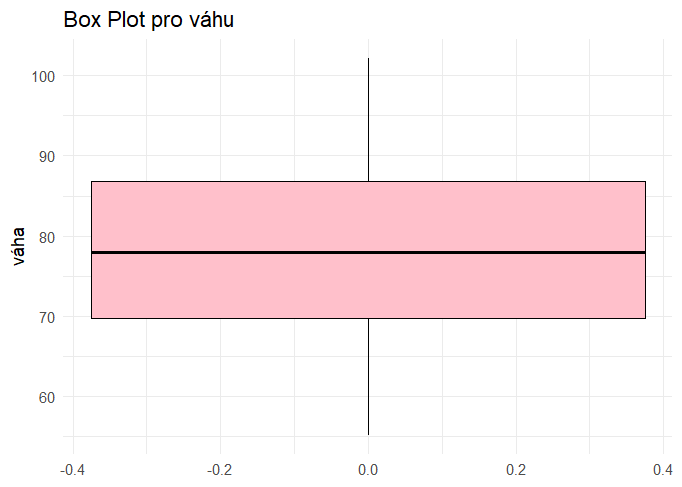
\includegraphics[width=0.8\textwidth]{boxplot.png}
    \caption{Boxplot pro váhu policistů}
    \label{fig:boxplot}
\end{figure}

\section{Závěr}
Analýza ukazuje, že váhy policistů jsou přibližně normálně rozdělené s mírnou pozitivní šikmostí. Variabilita dat je střední, s relativně nízkým výskytem extrémních hodnot. Robustní metody (medián, upravený průměr, Huberův odhad) potvrzují stabilitu dat.

\end{document}